
%%%%%%%%%%%%%%%%%%%%%%% file typeinst.tex %%%%%%%%%%%%%%%%%%%%%%%%%
%
% This is the LaTeX source for the instructions to authors using
% the LaTeX document class 'llncs.cls' for contributions to
% the Lecture Notes in Computer Sciences series.
% http://www.springer.com/lncs       Springer Heidelberg 2006/05/04
%
% It may be used as a template for your own input - copy it
% to a new file with a new name and use it as the basis
% for your article.
%
% NB: the document class 'llncs' has its own and detailed documentation, see
% ftp://ftp.springer.de/data/pubftp/pub/tex/latex/llncs/latex2e/llncsdoc.pdf
%
%%%%%%%%%%%%%%%%%%%%%%%%%%%%%%%%%%%%%%%%%%%%%%%%%%%%%%%%%%%%%%%%%%%


\documentclass[runningheads,a4paper]{llncs}


\usepackage{amssymb}
\usepackage{caption}
\usepackage{subcaption}
\captionsetup{compatibility=false}
\usepackage{algorithm}
\usepackage{algorithmic}
\usepackage{array}
\setcounter{tocdepth}{3}
\usepackage{graphicx}
\usepackage[margin=2.5cm]{geometry}

\usepackage{url}
\newcommand{\keywords}[1]{\par\addvspace\baselineskip
\noindent\keywordname\enspace\ignorespaces#1}

\begin{document}

\mainmatter  % start of an individual contribution

% first the title is needed
\title{Optimistic Concurrency Control in a Distributed NameNode Architecture for Hadoop Distributed File System}

% a short form should be given in case it is too long for the running head
\titlerunning{Optimistic Concurrency Control in a Distributed NameNode Architecture for Hadoop Distributed File System}

% the name(s) of the author(s) follow(s) next
%
% NB: Chinese authors should write their first names(s) in front of
% their surnames. This ensures that the names appear correctly in
% the running heads and the author index.
%
%
\author{Qi Qi}
\authorrunning{Optimistic Concurrency Control in a Distributed NameNode Architecture for Hadoop Distributed File System}
% (feature abused for this document to repeat the title also on left hand pages)
\institute{Instituto Superior T\'{e}cnico - IST (Portugal) \\ Royal Institute of Technology - KTH (Sweden)}
% the affiliations are given next; don't give your e-mail address
% unless you accept that it will be published

%
% NB: a more complex sample for affiliations and the mapping to the
% corresponding authors can be found in the file "llncs.dem"
% (search for the string "\mainmatter" where a contribution starts).
% "llncs.dem" accompanies the document class "llncs.cls".
%

\toctitle{Optimistic Concurrency Control in a Distributed NameNode Architecture for Hadoop Distributed File System}
\tocauthor{Qi Qi}
\maketitle


\begin{abstract}
The \textit{Hadoop Distributed File System} (HDFS) is the storage layer for Apache Hadoop ecosystem, persisting large data sets across multiple machines. However, the overall storage capacity is limited since the metadata is stored in-memory on a single server, called the \textit{NameNode}. The heap size of the NameNode restricts the number of data files and addressable blocks persisted in the file system.

The \textit{Hadoop Open Platform-as-a-service} (Hop) is an open platform-as-a-Service (PaaS) support of the Hadoop ecosystem on existing cloud platforms including Amazon Web Service and OpenStack. The storage layer of Hop, called the Hop-HDFS, is a highly available implementation of HDFS, based on storing the metadata in a distributed, in-memory, replicated database, called the \textit{MySQL Cluster}. It aims to overcome the NameNode's limitation while maintaining the strong consistency semantics of HDFS so that applications written for HDFS can run on Hop-HDFS without modifications.

Precedent thesis works have contributed for a transaction model for Hop-HDFS. From system-level coarse grained locking to row-level fine grained locking, the strong consistency semantics have been ensured in Hop-HDFS, but the overall performance is restricted compared to the original HDFS.

In this thesis, we first analyze the limitation in HDFS NameNode implementation and provide an overview of Hop-HDFS illustrating how we overcome those problems. Then we give a systematic assessment on precedent works for Hop-HDFS comparing to HDFS, and also analyze the restriction when using pessimistic locking mechanisms to ensure the strong consistency semantics. Finally, based on the investigation of current shortcomings, we provide a solution for Hop-HDFS based on optimistic concurrency control with snapshot isolation on semantic related group to improve the operation throughput while maintaining the strong consistency semantics in HDFS. The evaluation shows the significant improvement of this new model. The correctness of our implementation has been validated by 300+ Apache HDFS unit tests passing.
\keywords{HDFS, MySQL Cluster, Concurrency Control, Snapshot Isolation, Throughput}
\end{abstract}

\section{Introduction}
The \textit{Hadoop Distributed File System} (HDFS) is the storage layer for Apache Hadoop, which enables petabytes of data to be persisted on clusters of commodity hardware at relatively low cost~\cite{borthakur2008hdfs}. Inspired by the \textit{Google File System} (GFS)~\cite{ghemawat2003google}, the namespace, \textit{metadata}, is decoupled from data and stored in-memory on a single server, called the \textit{NameNode}. The file datasets are stored as sequences of blocks and replicated across potentially thousands of machines for fault tolerance.

Built upon the single namespace server (\textit{the NameNode}) architecture, one well-known shortcoming of HDFS is the limitation to growth~\cite{shvachko2010hdfs}. Since the metadata is kept in-memory for fast operation in NameNode, the number of file objects in the filesystem is limited by the amount of memory of a single machine.

The \textit{Hadoop Open Platform-as-a-service} (Hop) is an open platform-as-a-Service (PaaS) support of the Hadoop ecosystem on existing cloud platforms including Amazon Web Service and OpenStack. The storage layer of Hop, called the Hop-HDFS, is a highly available implementation of HDFS, based on storing the metadata in a distributed, in-memory, replicated database, called the \textit{MySQL Cluster}. It aims to overcome the NameNode's limitation while maintaining the strong consistency semantics of HDFS so that applications written for HDFS can run on Hop-HDFS without modifications.

However, in HDFS, the correctness and consistency of the namespace is ensured by atomic metadata mutation~\cite{shvachko2010hadoop}. In order to maintain the same level of strong consistency semantics, system-level coarse grained locking and row-level fine grained locking are adopted in precedent projects of Hop-HDFS, but the overall performance is heavily restricted compared to the original HDFS. Therefore, investigation for better concurrency control methods to improve the performance of Hop-HDFS is the main motivation of this thesis.

\subsection*{Contribution}
In this thesis, we contribute to the following three ways: First, we discuss the architectures of related distributed file systems, including Google File System, HDFS and Hop-HDFS. With focus on their namespace concurrency control schemes, we analyzes the limitation of HDFS's NameNode implementation. Second, we provide an overview of Hop-HDFS illustrating how it overcomes limitations in HDFS. With a systematic performance assessment between Hop-HDFS and HDFS, we discuss the current shortcomings in Hop-HDFS, which motivates this thesis for a better concurrency control scheme. Third, we provide a solution for Hop-HDFS based on optimistic concurrency control with snapshot isolation on semantic related group to improve the operation throughput while maintaining the strong consistency semantics in HDFS. As a proof of concept, the evaluation shows the significant improvement of this new model. The correctness of our implementation has been validated by 300+ Apache HDFS unit tests passing.

\section{Background and Related Work}
\subsection{The Hadoop Distributed File System}
The \textit{Hadoop Distributed File System} (HDFS) is inspired by the Google File System. Initially, HDFS is built for Hadoop Map-Reduce computational framework. With the development of Hadoop ecosystem including HBase, Pig, Mahout, Spark, etc, HDFS becomes the storage layer for all these big data applications. While enabling petabytes of data to be persisted on clusters of commodity hardware at relatively low cost, HDFS aims to stream these large data sets at high bandwidth to user applications. Therefore, like GFS, HDFS is optimized for delivering a high throughput of data at the expense of latency~\cite{white2012hadoop}.

Similar to GFS, HDFS stores metadata and file data separately. The architecture of a HDFS cluster consists of a single \textit{NameNode}, multiple \textit{DataNodes}, and is accessed by multiple \textit{clients}. Files in HDFS are split into smaller blocks stored in \textit{DataNodes}. For fault tolerance, each block is replicated across multiple \textit{DataNodes}. The \textit{NameNode} is a single dedicated metadata server maintaining the namespace, access control information, and file blocks mappings to DataNodes. The entire namespace is kept in-memory, called the \textit{image}, of the \textit{NameNode}. The persistent record of \textit{image}, called the \textit{checkpoint}, is stored in the local physical file system. The modification of the namespace (\textit{image}), called the \textit{journal}, is also persisted in the local physical file system. Copies of the \textit{checkpoints} and the \textit{journals} can be stored at other servers for durability. Therefore, the \textit{NameNode} restores the namespace by loading the checkpoint and replaying the journal during its restart.

\subsection{Hadoop Open Platform-as-a-service and Hop-HDFS}
The \textit{Hadoop Open Platform-as-a-service} (Hop) is an open platform-as-a-Service (PaaS) support of the Hadoop ecosystem on existing cloud platforms including Amazon Web Service and OpenStack. The goal is to automate the installation of both HDFS and Apache YARN so that unsophisticated users can deploy the stack on the cloud easily by a few clicks from our portal website.

The storage layer of Hop, called the Hop-HDFS, is a new high available model for HDFS's metadata, aiming to overcome the major limitations of HDFS NameNode architecture: (1) the scalability of the namespace - the memory size restricts the storage capacity in the system; (2) the throughput problem - the throughput of the metadata operations is bounded by the ability of the single machine (NameNode); (3) the failure recovery - it takes a long time for the NameNode to restart since it needs to load the checkpoint and replay the edit logs from the journal into the memory.

The architecture of Hop-HDFS consists of multiple \textit{NameNodes}, multiple \textit{DataNodes}, a \textit{MySQL cluster} and is accessed by multiple \textit{clients} as shown in Figure~\ref{fig:hophdfsar}. The design purpose for Hop-HDFS is to migrate the metadata from NameNode to an external distributed, in-memory, replicated database \textit{MySQL Cluster}. Therefore, the size of the metadata is not limited by a single NameNode's heap size so that the scalability problem can be solved. In Hop-HDFS, we have this \textit{multiple stateless NameNodes} architecture so that multiple-writers and multiple-readers are allowed to operate on the namespace to improve the throughput.

\begin{figure}[h!]
	\centering
	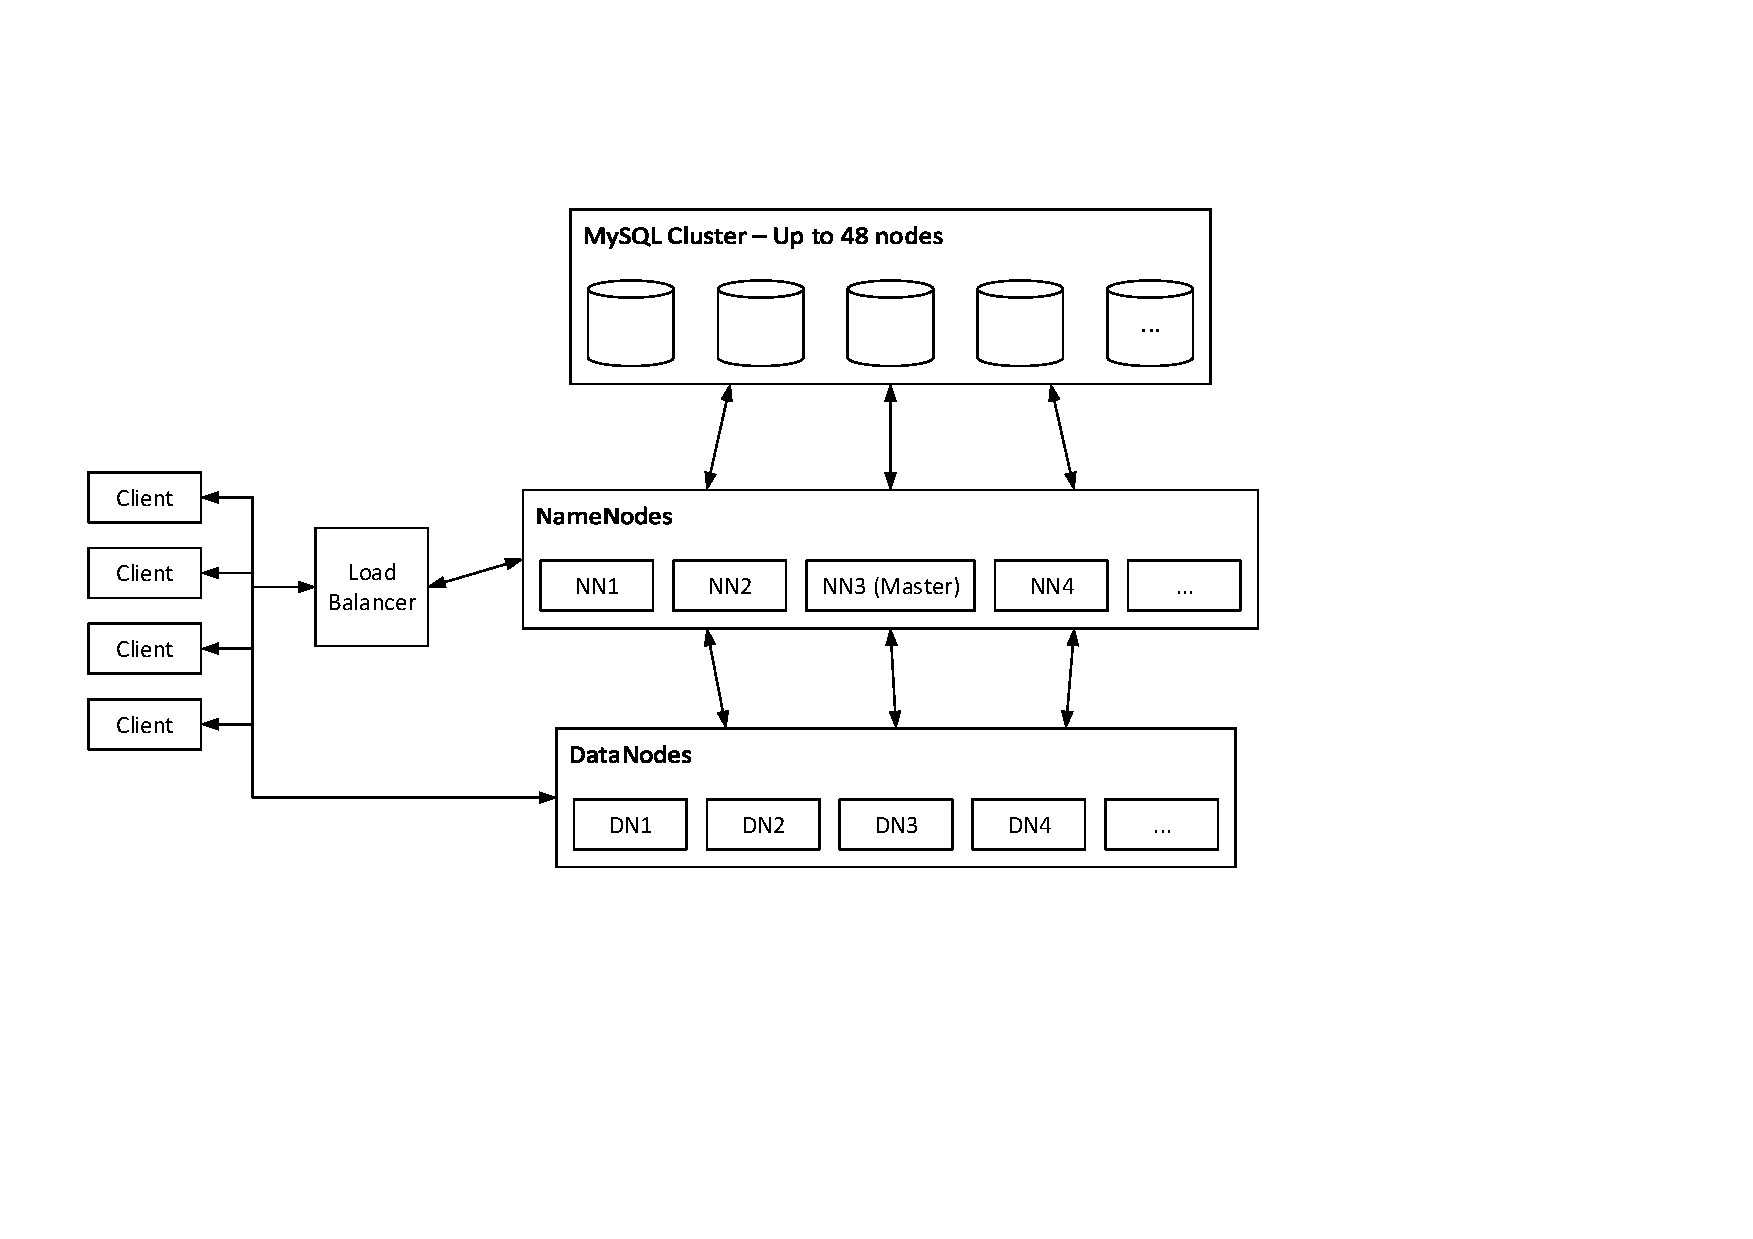
\includegraphics[scale=0.7]{HopHDFSArchitecture.pdf}
	\caption{The Architecture of Hop-HDFS}
	\label{fig:hophdfsar}
\end{figure}

Moreover, the fault tolerance of the metadata is handled by MySQL Cluster, which grantees high availability of 99.999\%. The \textit{checkpoint} and the \textit{journal} for namespace is removed as a result, which reduces the time on writing edit logs as well as restarting new NameNodes on namespace recovery. Note that we have a leader election process in this distributed NameNode architecture. The leader, \textit{master}, will be responsible for tasks like block reporting and statistic functions.

The size of the metadata for a single file object having two blocks (replicated three times by default) is 600 bytes. It requires 60 GB of RAM to store 100 million files in HDFS, 100 million files is also the maximum storage capacity for HDFS in practice. For MySQL Cluster, it supports up to 48 datanodes, which means that it can scale up to 12 TB in size with 256 GB RAM for each node in size. But conservatively, we assume that MySQL Cluster can support up to 3.072 TB for metadata with a data replication of 2, which means that Hop-HDFS can store up to 4.1 billion files. A factor of 40 times increase over Shvachko's estimate~\cite{shvachko2010hdfs} for HDFS from 2010.

\subsection{Namespace Concurrency Control and Performance Assessment in Hop-HDFS}
\subsubsection{Namespace Structure}
In HDFS, the namespace is kept in-memory as arrays and optimized data structure (like LinkedList) of objects with references for semantic constraints. Therefore, it has a \textit{directed tree structure}.

In Hop-HDFS, the namespace is stored into tables of MySQL Cluster database, so all INode objects are represented as individual row records in a single \textit{inodes table}. In order to preserve the directed tree structure, we add an id column and a parent\_id column to each row of in \textit{inodes table}. Therefore, the graphical representation of the filesystem hierarchy for INodes is like Figure~\ref{fig:hoptreeA}. The table representation in the database is like Table~\ref{table:hoptreeTableA}.

\begin{figure}[h]
	\centering
	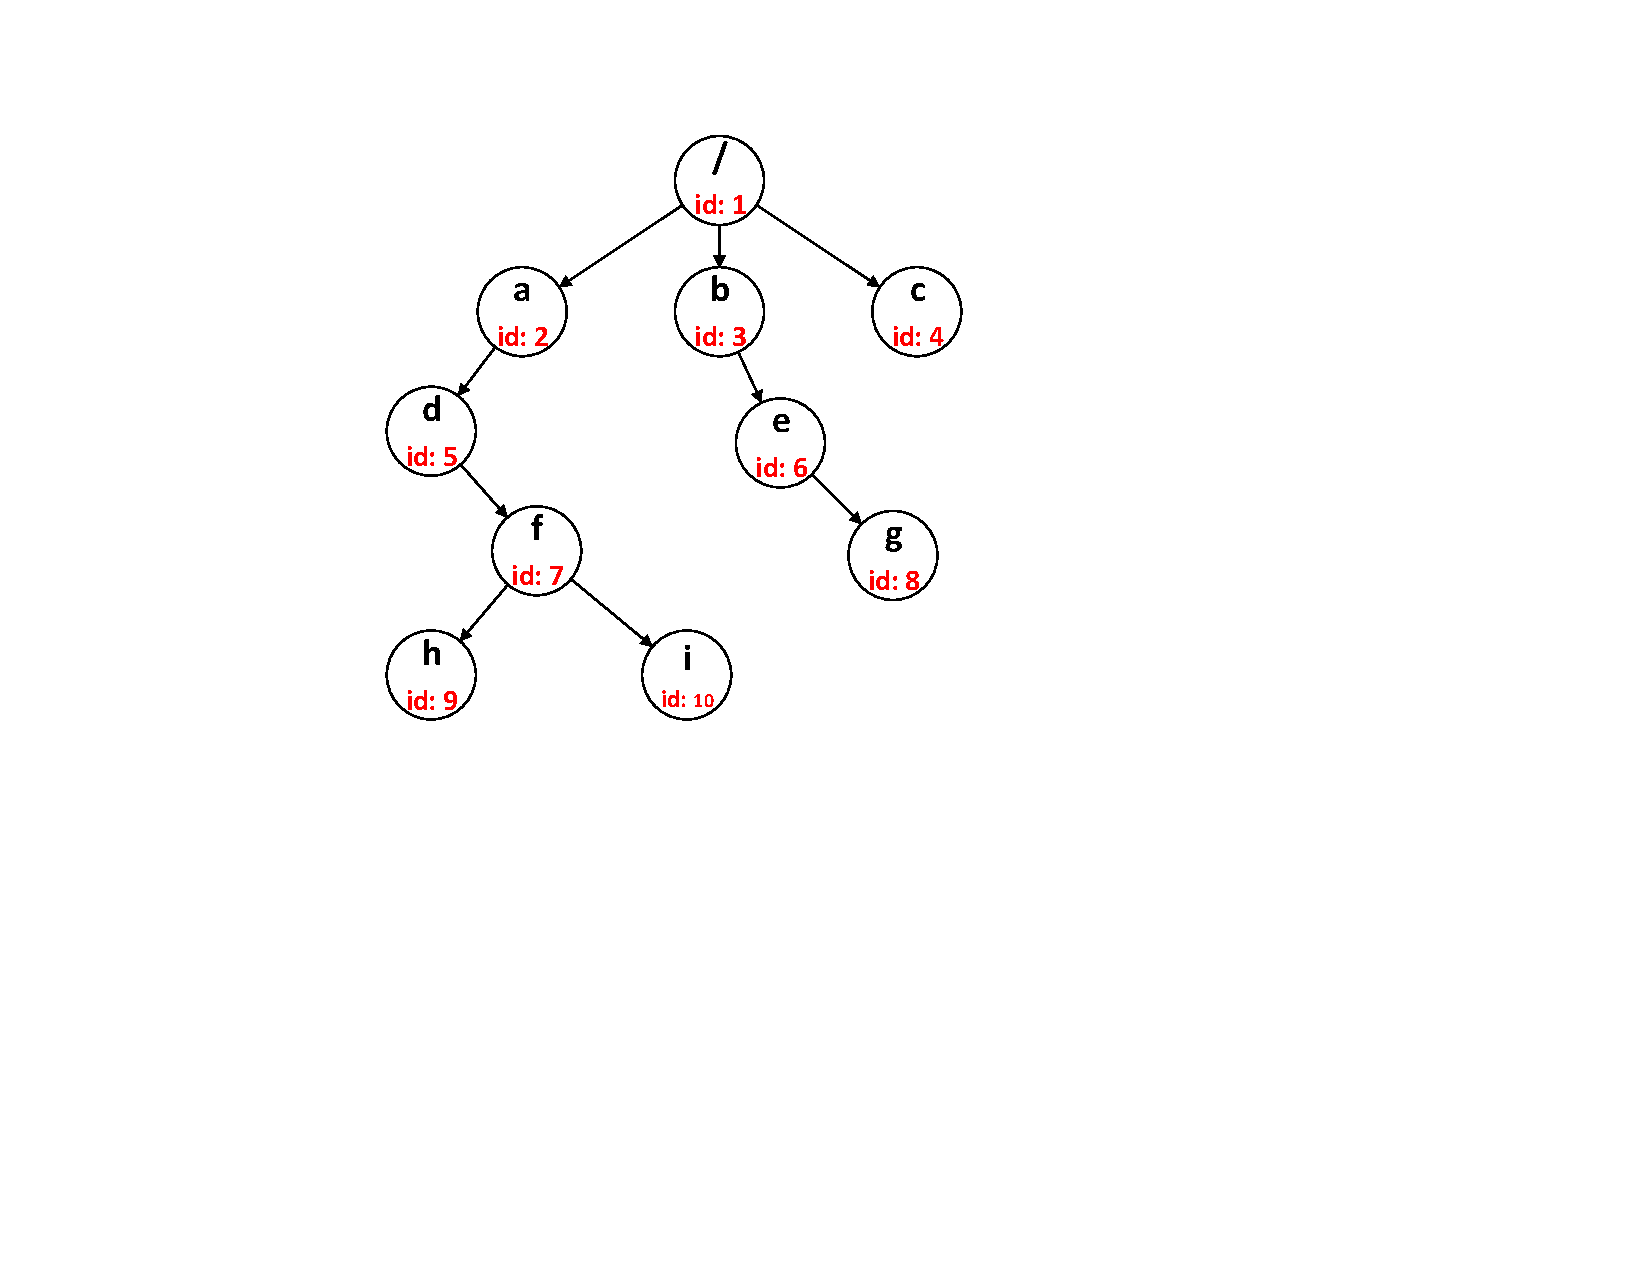
\includegraphics[scale=0.7]{hoptree.pdf}
	\caption{Filesystem Hierarchy with ID for INodes in Hop-HDFS}
	\label{fig:hoptreeA}
\end{figure}

\begin{table}[h]
	\centering
	\begin{tabular}{|c|c|c|c|}
		\hline
		\textbf{id} & \textbf{parent\_id} & \textbf{name} & \textbf{other parameters...} \\ \hline
		1 & 0 & / & ... \\ \hline
		2 & 1 & a & ... \\ \hline
		3 & 1 & b & ... \\ \hline
		4 & 1 & c & ... \\ \hline
		5 & 2 & d & ... \\ \hline
		6 & 3 & e & ... \\ \hline
		7 & 5 & f & ... \\ \hline
		8 & 6 & g & ... \\ \hline
		9 & 7 & h & ... \\ \hline
		10 & 7 & i & ... \\ \hline
	\end{tabular}
	\caption{INode Table for Hop-HDFS}
	\label{table:hoptreeTableA}
\end{table}

Since the \textit{id} is unique and atomically generated for INodes in each new transaction, the \textit{Primary Key} for the table is $<$name, parent\_id$>$ pair. Because the INode \textit{id} is not known beforehand on the application side, but the $<$name, parent\_id$>$ pair is known since it can be resolved from the path string. Therefore, data rows can be looked up by the $<$name, parent\_id$>$ pair \textit{Primary Key} directly from database on the application side. With the \textit{id} and \textit{parent\_id} relationship, the hierarchy will be constructed correctly from the data rows to in-memory objects used by the name system.

\subsubsection{Namespace Concurrency Control}
In the first version of Hop-HDFS~\cite{wasif2012distributed} (also named as KTHFS), the main task is to migrate the metadata from memory to MySQL Cluster. Therefore, it still depends on the system-level lock in HDFS NameNode (fsLock in \textit{FSNamesystem} - \textit{ReentrantReadWriteLock} to serialize the operations and maintain the semantics. This becomes a big problem since the network latency between NameNode and database is far more larger than it was when operated in-memory in original HDFS. Hence, each operation will take a long time lock on the name system. The throughput heavily decreases. A fine grained locking scheme is needed to improve the concurrency.

In the second version of Hop-HDFS~\cite{peiro2013maintaining} (also named as KTHFS), it adopts a fine-grained row-level locking mechanism to improve the throughput while maintaining the strong consistency semantics. It uses transactions with \textit{Pessimistic Concurrency Control} (PCC) to ensure the safety and progress of metadata operations. Based on a hierarchical concurrency model, it builds a \textit{directed acyclic graph} (DAG) for the namespace. Metadata operation that mutates the DAG either commit or abort (for partial failures) in a single transaction. Besides, \textit{implicit locking}~\cite{gray1976granularity} is used to lock on the root of a subtree in a transaction, which implicitly acquires locks on all the descendants, so that the strong consistent semantics from original HDFS can be maintained.

\subsubsection{Limitations}

There are two major limitations in this locking scheme:

1) It lowers the concurrency when multiple transactions try to mutate different descendants within the same subtree. Only one writer is allowed to work on INodes under one directory due to the implicit lock (Write Lock) for the parent directory. For example, if transaction Tx1 wants to mutate INode \textit{h}, and another transaction Tx2 wants to mutate INode \textit{i} concurrently in Figure~\ref{fig:hoptreeA}, Tx1 will take a parent lock on INode \textit{f} first and then perform operations. No more transactions can work under INode \textit{f} at the moment. Tx2 will be blocked by the implicit lock until Tx1 commits. See Table~\ref{table:hoplockTableA}.

2) There is un-avoided duplicated database round trips overhead. It takes two transactions to finish the implicit locking. The first transaction is used to resolve the path in the database so that we know which rows existed in the database so that the INode's parent directory can be taken the implicit write lock in the second transaction, or last existing INode directory can be taken the implicit write lock if the path is not full resolved(HDFS will build up the missing intermediate INodeDirectories). For example, if transaction Tx1 wants to mutate INode \textit{h} in Figure~\ref{fig:hoptreeA}, in the first database round trip, it needs to resolve the path to see if the related rows of INode\textit{ /, a, d, f, h} are all in the database. If yes, in the second database round trip, INode\textit{ /, a, d} will be taken Read Locks~\footnote{The third version of Hop-HDFS is trying to Replace Read Lock to Read\_Committed for this PCC scheme} and the INode \textit{f} will be taken a Write Lock; if no, the last existing INode will be taken a Write Lock while others will be taken Read Locks.

\begin{table}[h]
	\centering
	\begin{tabular}{|c|c|c|c|c|}
		\hline
		\textbf{id} & \textbf{parent\_id} & \textbf{name} & \textbf{Locks by Tx1} & \textbf{Locks by Tx2} \\ \hline
		1 & 0 & / & Read Lock & Read Lock \\ \hline
		2 & 1 & a & Read Lock & Read Lock \\ \hline
		3 & 1 & b & ~ & ~ \\ \hline
		4 & 1 & c & ~ & ~ \\ \hline
		5 & 2 & d & Read Lock & Read Lock\\ \hline
		6 & 3 & e & ~ & ~ \\ \hline
		7 & 5 & f  & Write Lock & Write Lock \textbf{(Blocked!)} \\ \hline
		8 & 6 & g & ~ & ~ \\ \hline
		9 & 7 & h (Mutated by Tx1) & Write Lock (Implicit) & Write Lock (Implicit) \textbf{(Blocked!)}\\ \hline
		10 & 7 & i (Mutated by Tx2) & Write Lock (Implicit) & Write Lock (Implicit)  \textbf{(Blocked!)}\\ \hline
	\end{tabular}
	\caption{Implicit Lock Table in Hop-HDFS}
	\label{table:hoplockTableA}
\end{table}

\subsubsection{Namespace Operation Performance Assessment}
\label{subsub:exp}
Here we will give the namespace operation performance assessment between the second version (PCC version) of Hop-HDFS and original HDFS under single NameNode. All the tests in this chapter are performed under same the experimental testbed described in Section~\ref{sec:eva}.

We aims to give a performance comparison between HDFS and PCC. Since the workload is generated from a single machine by the \textit{NNThroughtBenchmark}~\cite{shvachko2010hdfs}, we set the number of operations to be 100 and the number of threads to be 3. For operations \textit{create, delete and rename}, the total number of files involved is 100. They are placed under 4 different directories equally. For operation \textit{mkdirs}, the total number of directories created is 100 and they are also placed under 4 different directories equally. See Table~\ref{table:nntpbb} for the operation performance comparison between HDFS and PCC.

We find that the throughput of \textit{mkdirs} in PCC is 64.9 \% of HDFS, while others are all less than 30\%. The reason why the performance of \textit{create, delete and rename} is worse is because they involve multiple NameNode primitive operations. For example, to finish the \textit{create} operations, it takes two NameNode primitive operations (two transactions): \textit{startFile} and \textit{completeFile}. Since each NameNode primitive operation is implemented as a single transaction, the more primitive operations involved, the more parent write locks will be, which means that more transactions will be blocked.

\begin{table}[h]
	\centering
	\begin{tabular}{|c|c|c|c|c|}
		\hline
		\textbf{Operations per Second} & \textbf{create} & \textbf{mkdirs} & \textbf{delete} & \textbf{rename} \\ \hline
		HDFS                           & 609             & 636             & 833             & 869             \\ \hline
		PCC                 & 188             & 413             & 242             & 132             \\ \hline
		PCC / HDFS              & 30.9\%          & 64.9\%          & 29.1\%          & 15.2\%          \\ \hline
	\end{tabular}
	\caption{Operation Performance Comparison between HDFS and PCC}
	\label{table:nntpbb}
\end{table}

The worst case in PCC happens when all concurrent operations try to work under the same directory. Even though they mutate different INodes, all handling transactions will put a parent directory write lock to block each other. Therefore, the parent directory becomes a contention point. We design a test for the parent directory contention assessment. We build a thread pool with size 1024 for clients. We have three tests with 1000, 10000 and 100000 concurrent clients separately. Each client creates (\textit{mkdirs()}) one sub-directory. All these sub-directories are different, but they are all created under the same parent directory. The parent directory is the contention point in each task. We measure the elapsed time to finish all the concurrent creation tasks in each test.

As we can see from Table~\ref{table:hdfsPCCparentA}, it takes 4 - 5 more times in PCC to finish all these tasks compared to HDFS. However, when the size of concurrent tasks increases, this ratio decreases. Because under heavy workload, the edit logs in HDFS degrade the NameNode performance. Since there is no edit logging and check pointing part in Hop-HDFS, it works more efficiently than HDFS.

\begin{table}[h]
	\centering
	\begin{tabular}{|c|c|c|c|}
		\hline
		\textbf{Num. of Concurrent Creation} & \textbf{1000} & \textbf{10000} & \textbf{100000} \\ \hline
		HDFS                                 & 0.82s         & 7.83s          & 77.13s          \\ \hline
		PCC                       & 4.35s         & 36.74s         & 332.36s         \\ \hline
		PCC / HDFS                           & 530.5\%       & 469.2\%        & 430.9\%         \\ \hline
	\end{tabular}
	\caption{Parent Directory Contention Assessment between HDFS and PCC}
	\label{table:hdfsPCCparentA}
\end{table}

Note that the tests performed in this chapter is based on single NameNode. The multi-NameNode architecture in Hop-HDFS will help to improve the overall throughput.


\section{Solution}
The solution we propose to improve the throughput can be summarized as \textit{Optimistic Concurrency Control with Snapshot Isolation on Semantic Related Group}. The solution algorithm consists of the following four phases. \textbf{(1) Read Phase}: resolving the semantic related group and cache the snapshot copy within the handling transaction. \textbf{(2)Execution Phase}: transaction read/write operations are performed on its own snapshot and never fetch data from database. \textbf{(3)Validation Phase}: snapshot's related data rows are fetched from the database. If their versions all match with the snapshot copy, go to update phase; else, abort and retry current transaction.\textbf{(4)Update Phase}: update related data in the database table. Abort and retry transactions if the instance already exists in the database for "new" data. For successful updates, the versions of the modified rows will be increased by 1.

\subsection{Resolving the Semantic Related Group}
Resolving the semantic related group for each transaction is the fundamental step to preclude \textit{anomalies} in our implementation. The \textit{constraint violation}~\cite{berenson1995critique} between individual data is formed within a semantic related group. In Hop-HDFS, each metadata operation is implemented as a single transaction running by a worker thread. Any metadata operation related to the namespace will have one or two input parameters, called \textit{Path}.

Each \textit{Path} object is related to a string representation of the "/" based absolute path name. For example, in Figure~\ref{fig:hoptreeA}, the path for INode \textit{h} is: \textbf{h: \{/-$>$a-$>$d-$>$f\}}. In other words, when mutating INode \textit{h}, all the semantic constraint can be found within INodes \textit{/, a, d, f}. With this knowledge, we can maintain the strong consistency semantics in original HDFS.

For each row in \textit{inodes table}, the $<$name, parent\_id$>$ pair is the \textit{Primary Key}. With the full path string, we can iteratively resolve its semantic related rows by primary key lookups directly from database as shown in Table~\ref{table:semanticrelatedTableA}.

\begin{table}[h]
	\centering
	\begin{tabular}{|c|c|c|c|c|}
		\hline
		~ & \textbf{id} & \textbf{parent\_id} & \textbf{name} & \textbf{other parameters...} \\ \hline
		Related * & 1 & 0 & / & ... \\ \hline
		Related * & 2 & 1 & a & ... \\ \hline
		~ & 3 & 1 & b & ... \\ \hline
		~ & 4 & 1 & c & ... \\ \hline
		Related * & 5 & 2 & d & ... \\ \hline
		~ & 6 & 3 & e & ... \\ \hline
		Related * & 7 & 5 & f & ... \\ \hline
		~ & 8 & 6 & g & ... \\ \hline
		Selected \checkmark & 9 & 7 & h & ... \\ \hline
		~ & 10 & 7 & i & ... \\ \hline
	\end{tabular}
	\caption{Table Representation for the Semantic Related Group}
	\label{table:semanticrelatedTableA}
\end{table}

\subsection{Per-Transaction Snapshot Isolation}

As we mentioned before, MySQL Cluster supports only the READ COMMITTED transaction isolation level, which means that the committed results of write operations in transactions will be exposed by reads in other transactions. Within a long running transaction, it could read two different versions of data, known as \textit{fuzzy read}, and it could also get two different sets of results if the same query is issued twice, known as \textit{phantom read}.

\textit{Snapshot isolation} guarantees that all reads made within a transaction see a consistent view of at the database. At the beginning of the transaction, it reads data from a snapshot of the latest committed value. During transaction execution, reads and writes are performed on the this snapshot.

In commercial database management systems, like Microsoft SQL Server, Oracle, etc, \textit{snapshot isolation} is implemented within multi version concurrency control (MVCC)~\cite{berenson1995critique} on database server side. However, we need to implement snapshot isolation on the application side since MySQL Cluster supports only the READ COMMITTED isolation level.

After resolving the semantic related group, we take a snapshot on selected rows as well as all related rows of the committed values from database. This snapshot will be cached in-memory within its transaction. Each transaction will have its own copy of snapshot during the lifetime. All transaction operations will be performed on its own snapshot. Therefore, we called it Per-Transaction Snapshot Isolation.

\subsubsection{Fuzzy Read and Phantom Read are Precluded}
Before validation phase, the transaction will never fetch any data from database since it has all the semantic related rows in the cached snapshot. Therefore, the snapshot provides a consistent view of data for each transaction from read phase until validation phase. Hence: \textit{1. Fuzzy Read} is precluded by \textit{snapshot isolation}: Transactions read from snapshot instead of database, not affected by the value committed by others. \textit{2. Phantom Read} is also precluded by \textit{snapshot isolation on Semantic Related Group}: Transactions snapshot the semantic related group of after the operation. So if same operation peformed, it is not affected by the value committed by others since it operate from the snapshot.

\subsection{ClusterJ and Lock Mode in MySQL Cluster}
\textit{ClusterJ} is a Java connector based on object-relational mapping persistence frameworks to access data in MySQL Cluster. It doesn't depend on the MySQL Server to access data in MySQL Cluster as it communicates with data nodes directly, which means that ClusterJ can perform some operations much more quickly.

Unlike \textit{Two-Phase Locking} (2PL), there are three lock modes in MySQL Cluster. \textbf{(1) SHARED} (Read Lock, RL): Set a shared lock on rows; \textbf{(2) EXCLUSIVE} (Write Lock, WL): Set an exclusive lock on rows; \textbf{(3) READ\_COMMITTED} (Read Committed, RC): Set no locks but read the most recent committed values. For \textit{Read\_Committed}, it is implemented for consistent nonlocking reads, which means that a fresh committed snapshot of data row is always presented to a query of database, regardless of whether Shared Lock or Exclusive Lock are taken on the current row or not.

\subsection{Optimistic Concurrency Control}

Our algorithm is based on \textit{Optimistic Concurrency Control} (OCC) method to improve the overall read/write performance. Transactions are allowed to perform operations without blocking each other with optimistic methods. Concurrent transactions need to pass through a \textit{validation phase} before committing, so that the serializability is not violated. Transactions will abort and restart if they fail in the \textit{validation phase}. OCC is the key approach so that the parent directory lock is not needed in Hop-HDFS. Hence, transactions can operate under the same directory concurrently.

In \textit{read phase}, transactions use \textit{Read\_Committed Lock Mode} to fetch semantic related group as snapshots and cache them in-memory for their own use without being blocked. In \textit{validation phase}, transactions will fetch the modified rows using \textit{Exclusive Lock} and fetch the semantic related rows using \textit{Shared Lock}. Then they compare the fetched values and the snapshot copy in the cache for their \textit{versions}. If versions are all the same, go to \textit{update phase}. If not, abort current transaction, wait for a random milliseconds, and retry a new transaction from \textit{read phase}. Note that using \textit{Shared Lock} to fetch semantic related rows can guarantee a consistent view in database until the transaction commits while allowing other Shared Locks taken on the same rows for their validation phase.

\subsubsection{Write Skew is Precluded} The \textit{Write Skew} anomaly is precluded by the validation phase on the snapshot of semantic related group in OCC, because constraint violation on all related data rows will be checked before transaction committed.

\subsection{Total Order Update, Abort and Version Increase in Update Phase}
We have a total order update rule in update phase so that dead lock will not occur by lock cycle. If multiple rows needed to be during update phase, they will be sorted first by the \textit{id} value. Then they will be updated in ascending order according by \textit{ids}. Since we can not take an Exclusive lock on the "new" row which not yet exists in the database, multiple transactions may try to persist "new" rows with the same \textit{Primary Key}, and one might be overwritten by the other. Using \textit{makePersistent()} function in ClusterJ can throw exception if the instance already exists in the database. Finally, for successful updates, the versions of the modified rows will be increased by 1.
\subsection{Pseudocode of the Complete Algorithm}
See Algorithm~\ref{algo:pseudocodeA}.
\begin{algorithm}[!h]
	\caption{Pseudocode of the Complete Algorithm \\ Optimistic Concurrency Control with Snapshot Isolation on Semantic Related Group}
	\label{algo:pseudocodeA}
	\begin{algorithmic}[1]
		\STATE {\textbf{init:} restart = \TRUE, try = 0, path = operation.src, TotalRetry = 10}
		
		\WHILE{restart \AND try $<$ TotalRetry}
		\STATE {restart = \FALSE}
		\STATE {try += 1}
		\STATE {tx.snapshot.clear()}
		\STATE {tx.begin()}
		\STATE {\textit{\textbf{/* 1. Read Phase */}}}
		\STATE {tx.lockMode(\textit{Read\_Committed})}
		\STATE {tx.snapshot = resolve\_semantic\_related\_group(path)}
		\STATE {\textit{\textbf{/* 2. Execution Phase */}}}
		\STATE {operation\_performTask(tx.snapshot) // HDFS operation performs on its snapshot}
		\STATE {\textit{\textbf{/* 3. Validation Phase */}}}
		\STATE {tx.lockMode(\textit{Shared})}
		\STATE {relatedRows\_DataBase = batchRead\_Database(tx.snapshot)}
		\STATE {tx.lockMode(\textit{Exclusive})}
		\STATE {modifiedRows\_DataBase = batchRead\_Database(tx.snapshot)}
		\IF{versionCompare(relatedRows\_DataBase, tx.snapshot) $==$ \TRUE \textbf{ and} versionCompare(modifiedRows\_DataBase, tx.snapshot) $==$ \TRUE}
		\STATE {\textit{\textbf{/* 4. Update Phase */}}}
		\STATE {operation.modifiedRows.version+=1}
		\STATE {total\_order\_sort(operation.modifiedRows)}
		\IF{batchPersist\_Database(operation.modifiedRows) \textbf{success}}
		\STATE {tx.commit()}
		\STATE {return \textbf{SUCCESS} // Return HDFS Operation Success}
		\ELSE
		\STATE {tx.abort()}
		\STATE{waitForRandomMilliseconds()}
		\STATE{retry = \TRUE}
		\ENDIF
		\ELSE
		\STATE {tx.abort()}
		\STATE{waitForRandomMilliseconds()}
		\STATE{retry = \TRUE}
		\ENDIF
		\ENDWHILE
		
		\STATE {return \textbf{FAIL} // Return HDFS Operation}
	\end{algorithmic}
\end{algorithm}

\section{Evaluation}
\label{sec:eva}
The goal of this chapter is to proof that our OCC model performs better than PCC. As a proof of concept, we implemented the OCC version for the operation \textit{mkdirs} and also give a detailed evaluation on it compared with the PCC version. For this purpose, we concern about the execution time (elapsed time) needed to finish all the concurrent tasks.

Testbed Setup: The MySQL Cluster consists of six data nodes connected by 1 Gigabit LAN. Each data node has an Intel Xeon X5660 CPU at 2.80GHz, and contributes 6 GB RAM (5 GB Data Memory + 1 GB Index Memory) separately. Therefore, the total available memory for the cluster is 36 GB. The number of data replicas is 2. The maximum concurrent transactions is 10000 for each data node, and the inactive timeout for each transaction is 5 seconds. To avoid any communication overhead caused by RPC connections and serialization, we run the NameNode and Clients on the same machine with Intel i7-4770T CPU at 2.50GHz and 16 GB RAM. This machine is connected with the MySQL Cluster data nodes by 100 Megabits LAN.

\subsection{Parent Directory Contention Assessment}
This experiment is the same as described in Section~\ref{subsub:exp} but we expand it to include the results with OCC. Therefore, we have a full performance comparison here among HDFS, PCC and OCC. From Table~\ref{fig:hdfsPCCOCCparentA}, we can see that OCC significantly outperforms PCC by almost 70 \% on this concurrent write-write parent directory contention workload. Under heavy workload, the execution time is just 1.3 times of HDFS. Remember that this is just a single NameNode performance test. We believe that OCC can greatly outperform HDFS in our multiple NameNodes architecture.

\begin{table}[ht]
	\centering
	\begin{tabular}{|c|c|c|c|}
		\hline
		\textbf{Num. of Concurrent Creation}                                                 & \textbf{1000}   & \textbf{10000}  & \textbf{100000} \\ \hline
		HDFS                                                                                 & 0.82s           & 7.83s           & 77.13s          \\ \hline
		PCC                                                                                  & 4.35s           & 36.74s          & 332.36s         \\ \hline
		OCC                                                                                  & 1.36s           & 12.01s          & 103.23s         \\ \hline
		PCC / HDFS                                                                           & 530.5\%         & 469.2\%         & 430.9\%         \\ \hline
		OCC / HDFS                                                                           & 165.9\%         & 153.4\%         & 133.8\%         \\ \hline
		\textbf{\begin{tabular}[c]{@{}c@{}}OCC Improvement: \\ (PCC-OCC) / PCC\end{tabular}} & \textbf{68.7\%} & \textbf{67.3\%} & \textbf{68.9\%} \\ \hline
	\end{tabular}
	\caption{OCC Performance Improvement on Parent Directory Contention}
	\label{table:hdfsPCCOCCparentA}
\end{table}

\subsection{Read-Write Mixed Workload Assessment}

In this experiment, we did a test for a read-write mixed workload assessment while the parent directory is still the contention point for PCC. So we assume that OCC will still outperform PCC in this kind of workload. Similar to the experiment in Section~\ref{subsub:exp}, we have 1000, 10000 and 100000 concurrent clients' operations running under the same parent directory. But in each task, half of them will do the metadata read operation \textit{getFileStatus()}, while the other half will do the write operation \textit{mkdirs()}.

From Table~\ref{table:rwA}, we can see that OCC still significantly outperforms PCC by 65 \% on this concurrent read-write mixed workload.

\begin{table}[ht]
	\centering
	\begin{tabular}{|c|c|c|c|}
		\hline
		\textbf{Num. of Concurrent Creation}                                                 & \textbf{1000}   & \textbf{10000}  & \textbf{100000} \\ \hline
		PCC                                                                                  & 4.92s           & 50.69s          & 352.25s         \\ \hline
		OCC                                                                                  & 1.78s           & 15.31s          & 120.64s         \\ \hline
		\textbf{\begin{tabular}[c]{@{}c@{}}OCC Improvement: \\ (PCC-OCC) / PCC\end{tabular}} & \textbf{63.8\%} & \textbf{69.8\%} & \textbf{65.8\%} \\ \hline
	\end{tabular}
	\caption{OCC Performance Improvement on Read-Write Mixed Workload}
	\label{table:rwA}
\end{table}

\subsection{OCC Performance with Different Size of Conflicts}

When OCC conflicts happen, transactions will abort, wait for random milliseconds and retry. Eventually one transaction will success, and others will get updated values after retry and return RPC callbacks. Here we have 10000 concurrent operations running under the same parent directory. Each operation creates only one sub-directory. Some of them will success and some others will fail due to conflicts. These operations will try to create same sub-directories in different numbers from 1 (all conflicts), to 10000 (no conflicts). Therefore, we have different size of conflicts.

From Table~\ref{table:conflictsA}, we can find that the maximum OCC performance decrease is only 23.7\% when 100 \% of the operations conflict: $(14.53-11.75) \div 11.75 = 23.7\%$. Besides, we find that the OCC performance decrease rate grows very slowly after conflict size 10\%. From conflict size 10\% to conflict size 100 \%, the performance decrease rate only grows from 20.1 \% to 23.7 \%.

\begin{table}[ht]
	\centering
\begin{tabular}{|c|c|c|c|}
	\hline
	\textbf{\begin{tabular}[c]{@{}c@{}}Total Num. of Sub-Directories \\ Created for 10000 Operations\end{tabular}} & \textbf{\begin{tabular}[c]{@{}c@{}}Conflict\\  Size\end{tabular}} & \textbf{\begin{tabular}[c]{@{}c@{}}Elapsed Time\\  (Second)\end{tabular}} & \textbf{\begin{tabular}[c]{@{}c@{}}Performance Decrease\\ Compared to Zero Conflict\end{tabular}} \\ \hline
	1                                                                                                              & 100\%                                                             & 14.53                                                                     & 23.7\%                                                                                            \\ \hline
	10                                                                                                             & 10\%                                                              & 14.11                                                                     & 20.1\%                                                                                            \\ \hline
	100                                                                                                            & 1\%                                                               & 13.51                                                                     & 15.0\%                                                                                            \\ \hline
	1000                                                                                                           & 0.1\%                                                             & 12.72                                                                     & 8.23\%                                                                                            \\ \hline
	10000                                                                                                          & 0\%                                                               & 11.75                                                                     & 0\%                                                                                               \\ \hline
\end{tabular}
	\caption{OCC Performance with Different Size of Conflicts}
	\label{table:conflictsA}
\end{table}

\subsection{Correctness Assessment}
The correctness of our OCC implementation for \textit{mkdirs()}~\footnote{other operations are PCC} has been validated by 300+ Apache HDFS 2.0.4 Alpha unit tests passing.

\section{Conclusion}
In this thesis, we provide a solution for Hop-HDFS based on optimistic concurrency control with snapshot isolation on semantic related group to improve the operation throughput while maintaining the strong consistency semantics in HDFS.

First, we discuss the architectures HDFS and Hop-HDFS. With focus on the namespace concurrency control schemes, we analyzes the limitation of HDFS's NameNode implementation and provide an overview of Hop-HDFS illustrating how we overcome those problems in the distributed NameNode architecture.

MySQL Cluster is selected to be the distributed in-memory storage layer for the metadata in Hop-HDFS due to its the high operation throughput and high reliability. However, the trade off is that the cluster storage engine of MySQL cluster supports only the \textit{READ COMMITTED} transaction isolation level. \textit{Anomalies} like fuzzy read, phantom, write skew will appear because the write results in transactions will be exposed to reads in different concurrent transactions without proper implementation.

Then, based on optimistic concurrency control with snapshot isolation on semantic related group, we demonstrate how concurrency is improved and anomalies - \textit{fuzzy read, phantom, write skew} are precluded, so that the strong consistency semantics in HDFS is maintained.

Finally, as a proof of concept, we implemented the OCC version for the operation \textit{mkdirs} and also give a detailed evaluation on it compared with the PCC version. Our solution outperforms previous work of Hop-HDFS up to 70 \%. Under heavy workload, the single NameNode performance of HDFS is just a slightly better than OCC. We believe that OCC can greatly outperform HDFS in Hop-HDFS multiple NameNodes architecture. The correctness of our implementation has been validated by 300+ Apache HDFS unit tests passing.

\subsection{Future work}
The result of our OCC solution is promising. Other operations in Hop-HDFS can also adopt the same algorithm to achieve better performance. Future evaluation on Hop-HDFS in multiple NameNodes architecture with OCC solution is needed to prove that it can achieve better performance than HDFS in single NameNode architecture.

\bibliography{reference}

\begin{thebibliography}{4}

\bibitem{borthakur2008hdfs} Borthakur, Dhruba. "HDFS architecture guide." HADOOP APACHE PROJECT http://hadoop. apache. org/common/docs/current/hdfs design. pdf (2008).

\bibitem{ghemawat2003google} Ghemawat, Sanjay, Howard Gobioff, and Shun-Tak Leung. "The Google file system." ACM SIGOPS Operating Systems Review 37, no. 5 (2003): 29-43.

\bibitem{shvachko2010hdfs} Shvachko, Konstantin V. "HDFS Scalability: The limits to growth." login 35, no. 2 (2010): 6-16.

\bibitem{shvachko2010hadoop} Shvachko, Konstantin, Hairong Kuang, Sanjay Radia, and Robert Chansler. "The hadoop distributed file system." In Mass Storage Systems and Technologies (MSST), 2010 IEEE 26th Symposium on, pp. 1-10. IEEE, 2010.

\bibitem{white2012hadoop} White, Tom. "Hadoop: The definitive guide." (2012).

\bibitem{wasif2012distributed} Wasif, Malik. "A Distributed Namespace for a Distributed File System." (2012).

\bibitem{peiro2013maintaining} Peiro Sajjad, Hooman, and Mahmoud Hakimzadeh Harirbaf. "Maintaining Strong Consistency Semantics in a Horizontally Scalable and Highly Available Implementation of HDFS." (2013).

\bibitem{gray1976granularity} Lorie, Raymond A., Gianfranco R. Putzolu, and Irving L. Traiger. "Granularity of locks and degrees of consistency in a shared data base." In IFIP Working Conference on Modelling in Data Base Management Systems, pp. 365-394. 1976.

\bibitem{berenson1995critique} Berenson, Hal, Phil Bernstein, Jim Gray, Jim Melton, Elizabeth O'Neil, and Patrick O'Neil. "A critique of ANSI SQL isolation levels." ACM SIGMOD Record 24, no. 2 (1995): 1-10.

\end{thebibliography}

\end{document}
